
\chapter{Writing \LaTeX}

This is the start of a chapter and gives some introduction before its first section.  This chapter describes basic \LaTeX{} you need to know.

%%%%%%%%%%%%%%%%%%%%%%%%%%%%%%%%%%%%%%%%%%%%%%%%%%%%%%%%%%%%%%%%%%%%
\section{Sectioning}
\label{sec:sectioning}

The following sectioning macros are available, ordered in descending
importance:

\begin{verbatim}
\chapter{A Chapter}
\section{A Section}
\subsection{A Sub Section}
\subsubsection{A Sub Sub Section}
\subsubsubsection{A Sub Sub Sub Section}
\end{verbatim}

Three-sub's is all you get.  
Consult with the technical editors if you feel finer grained
sectioning is required.
Starting from \verb|\subsection|, this produces the following:

\subsection{A Sub Section}
\subsubsection{A Sub Sub Section}
\subsubsubsection{A Sub Sub Sub Section}

Just after defining a chapter and any significant section a
\verb|\label| should be added so it can be referenced.
A label can be added later for a `'less significant'' section that
turns out to need one. You can label them all. 

For example:

\begin{verbatim}
\chapter{A Chapter}
\label{ch:a-chapter}

\section{A Section}
\label{sec:a-section}

\subsection{A Sub Section}
\label{subsec:a-subsection}
\end{verbatim}

See Section~\ref{sec:refs} for how to reference labeled sections.

%%%%%%%%%%%%%%%%%%%%%%%%%%%%%%%%%%%%%%%%%%%%%%%%%%%%%%%%%%%%%%%%%%%%
\section{Including Figures}
\label{sec:figures}

See Section~\ref{sec:figure-format} for guidelines on the graphics files themselves.
Any graphics element is included using this command:

\begin{verbatim}
\includegraphics[OPTIONS]{volume-VNAME/figures/myfigurefile}
\end{verbatim}

The file's extension may be optionally omitted.
The file is located relative to the top directory given in the guidance in Section~\ref{sec:files}, hence the (typically used) ``volume-VNAME/figures/'' preceding the filename.  This is because the tex file is pulled into \texttt{volume-VNAME.tex} and the figure is searched for relative to it.
The \texttt{OPTIONS} most likely used will be to scale the graphic to
a sensible size.  Examples:

\begin{verbatim}
\includegraphics[width=0.5\textwidth]{...}
\includegraphics[height=0.1\textheight]{...}
\end{verbatim}

Graphics should always be placed in \texttt{figure} environments and include reference label (see
section~\ref{sec:refs} for how to reference figures and tables) and a
caption.  Captions will be printed in the ``List of Figures''.  A
synopsis of a caption should be given in ``[]'' in order to make the
entries in the List of Figures brief and readable.  The synopsis doesn't need to describe it fully, just identify it clearly. Captions are to be listed below the graphic itself.

Here is an example of how to add a figure:
%  http://www-visualmedia.fnal.gov/VMS_Site/gallery/stillphotos/2007/0300/07-0329-14D.jpg

BRETT -- I WOULD MOVE THIS FIG INTO THE VOLUME'S FIGURES DIRECTORY AND USE THE PATH
volume-VNAME/figures/fermilab-aerial.jpg

\begin{verbatim}
\begin{figure}[h]
  \centering
  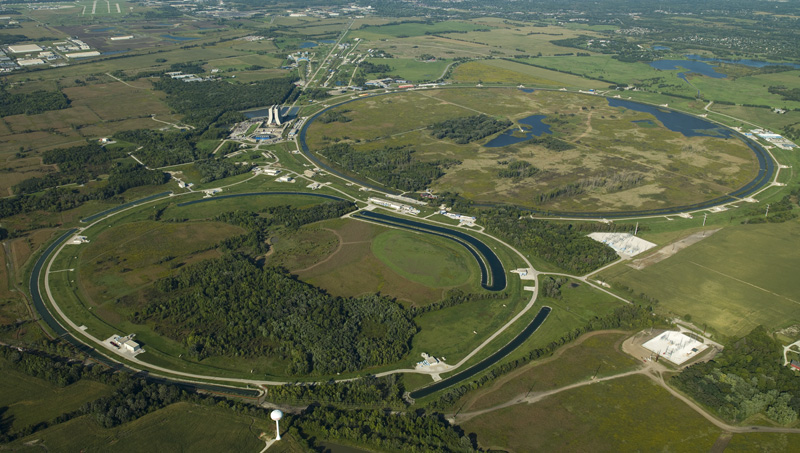
\includegraphics[width=\textwidth]{fermilab-aerial.jpg}
  \caption[Aerial photo of Fermilab]{An aerial photograph of Fermilab
    showing Wilson Hall and surrounding accelerator rings (Fermilab
    Visual Media Services). (Notice in the source file, caption is listed below includegraphics.)}
  \label{fig:fermilab-aerial}
\end{figure}
\end{verbatim}

\begin{figure}[h]
  \centering
  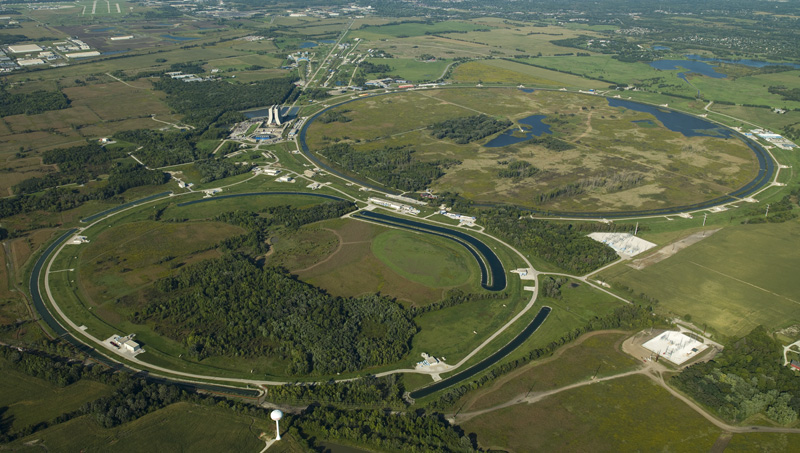
\includegraphics[width=\textwidth]{fermilab-aerial.jpg}
  \caption[Aerial Photo of Fermilab]{An aerial photograph of Fermilab
    showing Wilson Hall and surrounding accelerator rings (Fermilab
    Visual Media Services).}
  \label{fig:fermilab-aerial}
\end{figure}

%%%%%%%%%%%%%%%%%%%%%%%%%%%%%%%%%%%%%%%%%%%%%%%%%%%%%%%%%%%%%%%%%%%%
\section{Tables}
\label{sec:tables}

Tables (actually ``tabular'' environments in a table floating environment) are defined like:

WOULD IT MAKE SENSE TO USE THE SAME TABLE MACHINERY AS IN THE SCI OPP DOC? IT LOOKED NICE,
MIGHT BE MORE WORK THAN I REALLY WANT...

\begin{verbatim}
\begin{table}[h]
  \centering
  \caption[Table of things]{A table showing some things. (This caption is listed before the start of
  the tabular environment.)}
  \label{tab:things}
  \begin{tabular}[h]{|r|c|l|}
    \hline
    Column1 & Column2 & Column3 \\
    \hline
    thing1 & thing2 & thing 3 \\
    \hline
  \end{tabular}
  \caption[Table of things]{A table showing some things}
  \label{tab:things}
\end{table}
\end{verbatim}
\begin{table}[h]
  \centering
  \begin{tabular}[h]{|r|c|l|}
    \hline
    Column1 & Column2 & Column3 \\
    \hline
    thing1 & thing2 & thing 3 \\
    \hline
  \end{tabular}
\end{table}

Table captions should appear above the tables to which they refer -- opposite from figure captions.

%%%%%%%%%%%%%%%%%%%%%%%%%%%%%%%%%%%%%%%%%%%%%%%%%%%%%%%%%%%%%%%%%%%%
\section{Referencing}
\label{sec:refs}

Note: if you see a greyed out ``\textbf{LABEL: ``sec:refs''}'' just above this
line (or elsewhere in chapters, sections, figures, etc), it means this
document was built in draft mode.  These artifacts show up to help you know what label
was used to reference each particular thing.

Assume that any chapter, section or important sub-, subsub-,  section or
within any figure or table environment may need to be referenced
elsewhere in the text. As described in Section~\ref{sec:sectioning}, define a label (\verb|label{...}|
for these items.
Use the defined label in a \verb|\ref{...}| in order to
make reference to the chapter, section, figure, etc.  For example:

\begin{verbatim}
\chapter{Some Chapter}
\label{ch:some-chapter}

\subsection{Some Sub Section}
\label{subsec:some-sub-section}

...

As described in Chapter~\ref{ch:some-chapter} ...

As shown in Figure~\ref{fig:fermilab-aerial} ...
\end{verbatim}

When you reference a chapter, section, subsection, figure, table, etc., capitalize the word ``Chapter'' or whatever it is, e.g., ``as shown in Section~\ref{sec:plots}.''  Use the word ``Section'' even if it's a subsection or subsubsection, and use the tilde sign to keep the number on the same line as the word that precedes it.

Examples for figures and tables have been given above.  Here I
reference this section:~\ref{sec:refs}.  



